

%************************************************
\subsection{Consumer}

The \ndnrtcName{} architecture is receiver-driven, in which the consumer aims to achieve the following goals:
\begin{itemize}
\item fetch the latest data available in the network; 
\item choose the most appropriate media stream bandwidth from those  provided by the producer (by monitoring network conditions);
\item fetch (and, if necessary reassemble) media in the correct order for playback;
\item mitigate, as far as possible, the impact of network latency and packet drops on the viewer's quality of experience.
\end{itemize}

%************************************************
\subsubsection{Interest pipelining and Data buffering}

Media streams are packetized by the publisher, currently into segments that are less than the typical 1500 byte MTU of the current Internet. The consumer implements Interest pipelining and Data buffering (see Figure \ref{fig:consumer}) to fetch and reassemble video and audio data. An asynchronous Interest pipeline issues Interests for individual segment. Packet re-ordering and drops and latency fluctuations absorption are handled by the frame buffer, which re-arranges received frames in the playback order.
%%Sentence 3 of the previous paragraph could mean a few things as currently written.


%************************************************
\subsubsection{Frame fetching}

The consumer obtains the number of segments per frame from metadata in the first segment of the frame; however, to minimize latency, it should issue a pipeline of Interests simultaneously.  Therefore, at first, the consumer uses an estimate of the number of segments it must fetch for a given frame, issuing $M$ Interests (see Figure \ref{fig:pull}). If Interests arrive too early, they will be held in the producer's PIT and stay there until the frame is captured and packetized. We call the delay between interest arrival and availability of the media data the \textbf{generation delay}, $d_{gen}$. Once the encoded frame is segmented into $N$ segments and published, Interests $0 - M$ are answered and the Data returns to the requestor(s). Upon receiving the first data segment, the consumer knows the exact number of segments for the current frame, and issues $N - M$ more Interests for the missing segments, if any. These segments will be satisfied by data with no generation delay, as the frame has been published already by the producer. The time interval between receiving the very first segment and when the frame is fully assembled is represented by $d_{asm}$ and called \textbf{assembly time}. Note that for frames that are smaller than the estimate, some Interests may go unanswered; this is currently a tradeoff made to try to keep latency for the frame as a whole low. These Interests have low lifetimes, of about 300ms. 
 

\begin{figure}[t!]
\centering
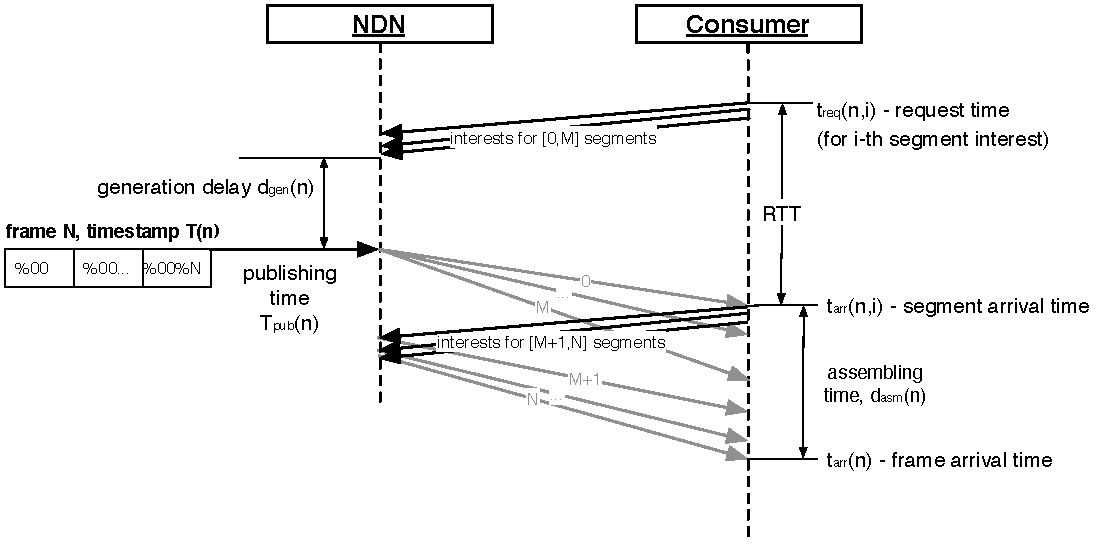
\includegraphics[width=0.5\textwidth]{frame-fetch}
\vspace{-18pt}
\caption{Fetching frame}
\label{fig:pull}
\end{figure}

Of course, additional round trips for requesting missing data segments increase overall frame assembly time and the possibility that the frame will be incomplete by the time it should be played back. This problem can be mitigated if the consumer is able to make more accurate estimates of the number of initial Interests. The latest versions of the library uses different namespaces for bitrates, and within each bit frame, for key frames and delta frames, making it straightforward for the consumer to keep interests outstanding for the next frame in each and to estimate the number of interests needed per frame, as the average number of segments varies greatly for different frame types. 
Additionally, it track the average number of segments per frame type, adapting its estimates over time. 

%% Is a similar process used for audio? 

\subsubsection{Buffering}

% Buffer:
% - re-ordering
% - added latency to mitigate network delays
% - extended defition:
% 	- pending frames
% 	- assembling frames
% - buffer-based retransmissions

As in sender-driven delivery, the consumer uses a ``jitter buffer" in order to manage out-of-order data arrivals and variations in network delay, and as a place to assemble segments into frames. However, the role of such a ``jitter buffer"  has some NDN-specific aspects. In sender-based video delivery, buffer slots can be allocated only when data arrives. A pull-based paradigm requires the consumer to request data by name explicitly, however. Therefore, after expressing an Interest, the consumers ``knows" that new data is coming, and a frame slot should be reserved in the buffer. Practically, this means that there will always be some number of reserved empty slots in the buffer. Thus, the \ndnrtcName{} jitter buffer's size is expressed in terms of two values: Its  \textit{playback size} is the playback duration of all complete ordered frames by the moment. %% WHAT DOES THIS MEAN? WHAT MOMENT? WHAT UNITS? 
Its \textit{estimated size} is \textit{playback size} + \textit{number of reserved slots} $\times$ 1/\textit{producer rate}.  % WHAT UNITS? 

The difference between estimated buffer size and playback size corresponds to the effective RTT, which we call $RTT^{\prime}$.  (This cannot be smaller than the actual network RTT value.) Minimizing $RTT^{\prime}$ indicates that consumer receives the most recent data for the leeast amount of outstanding Interests. %% NOT CLEAR WHAT THIS MEANS
Monitoring this value over times provides the consumer information on possible ``sync" status with the producer. %% HOW? 
For example, the consumer may use it during the fetching process, as will be discussed in the next section. 
%% Correct formatting for($RTT^{\prime}$)?

\subsubsection{Interest expression control}

A key challenge in a consumer-driven model for videoconferencing in a caching network is to ensure the consumer gets the latest data, without resorting to direct producer-consumer communication that would limit scaling. To get fresh data, the consumer cannot rely on using such flags as \textit{AnswerOriginKind} and \textit{RightMostChild}. The high rate of streaming data relative to network latency means there is no guarantee that the data satisfying those flags received by a consumer will be the most recent one. Instead, it is necessary to use other indicators to ensure that the consumer is requesting the most up-to-date stream data possible given its network connectivity. 

Our initial solution is to leverage the known segment publishing rate, which is available in stream-level metadata, and note that, under normal operation, old, cached samples are likely to be retrieved more quickly than new data.~\footnote{If the consumer is the \emph{only} consumer of the stream, its interests will go directly to the publisher, which also yields the correct behavior. A more complex challenge, for further study, is when segments are inconsistently cached in different ways along the path(s) that Interests take.} We define the interarrival delay ($D_{arr}$) as the time between receipt of successive samples at a given consumer. Delays in the most recent samples follow the publishers' generation pattern, but cached data will follow the Interest expression temporal pattern. Therefore, by monitoring inter-arrival delays of consecutive media samples and comparing them to the timing of Interest expression, consumers can estimate data freshness (see Figure \ref{fig:inter-arrival}).

%%The following sentences really don't make much sense: To get fresh data, which can be cached but should not be the newest available for the consumer's path, the consumer cannot rely only on using such flags as \textit{AnswerOriginKind} and \textit{RightMostChild}. The high frequency nature of streaming data makes no guarantees that the data satisfying those flags received by a consumer will be the most recent one.


\begin{figure}[t!]
\centering

\subfigure[Bursty arrival of cached data, which reflects interests expression pattern and indicates that the data is not the latest.]{\label{fig:cached}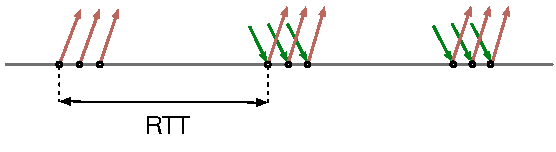
\includegraphics[width=0.4\textwidth]{arrival-cached}}\\
\subfigure[Periodic arrival of fresh data, reflects publishing pattern and sample rate.]{\label{fig:fresh}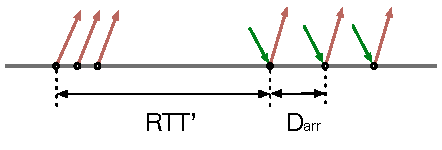
\includegraphics[width=0.35\textwidth]{arrival-fresh}}

\caption{Getting the latest data: arrival patterns for the cached and most recent data}
\label{fig:inter-arrival}
\end{figure}

During bootstrapping, the consumer ``chases" the producer and aims to exhaust network cache of historical (non-real time) segments. By increasing the number of outstanding Interests, the consumer ``pulls cached data" out of the network, unless the freshest data begin to arrive. In order to control Interest expression, a concept of $W$ (roughly an ``Interest window") is introduced (see Figure \ref{fig:w-concept}). It expresses Interests only when $W > 0$. At every moment, $W$ indicates how many outstanding Interests can be sent. Before the bootstrapping phase, the consumer initializes $W$ with a value which reflects the consumer's estimate of how many Interests are needed in order to exhaust network cache and reach the most recent data. 

\begin{figure}[t!]
\centering

\subfigure[$W$ concept]{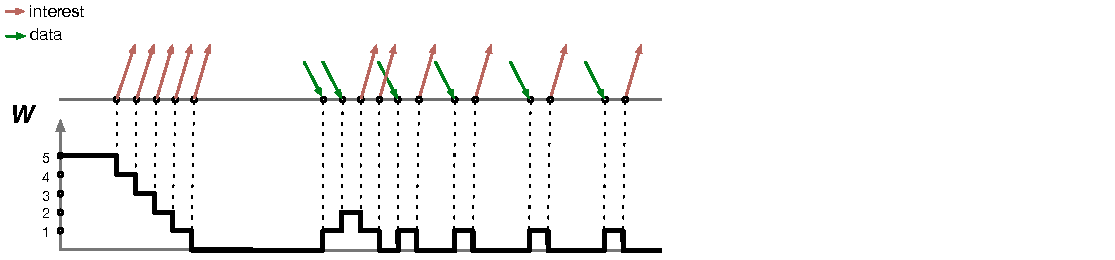
\includegraphics[width=0.35\textwidth]{w-concept}}
\subfigure[interests bursting ($W+3$)]{\label{fig:int-burst}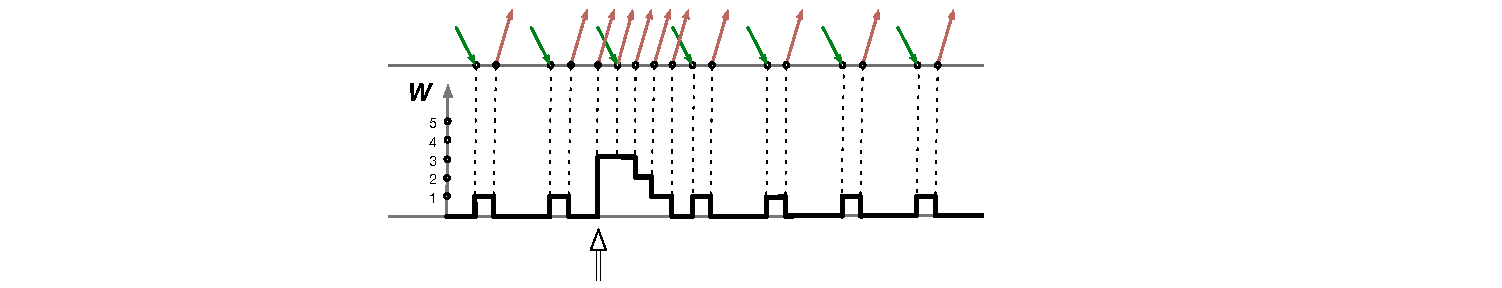
\includegraphics[width=0.35\textwidth]{int-burst}}
\subfigure[interests withholding ($W-3$)]{\label{fig:int-hold}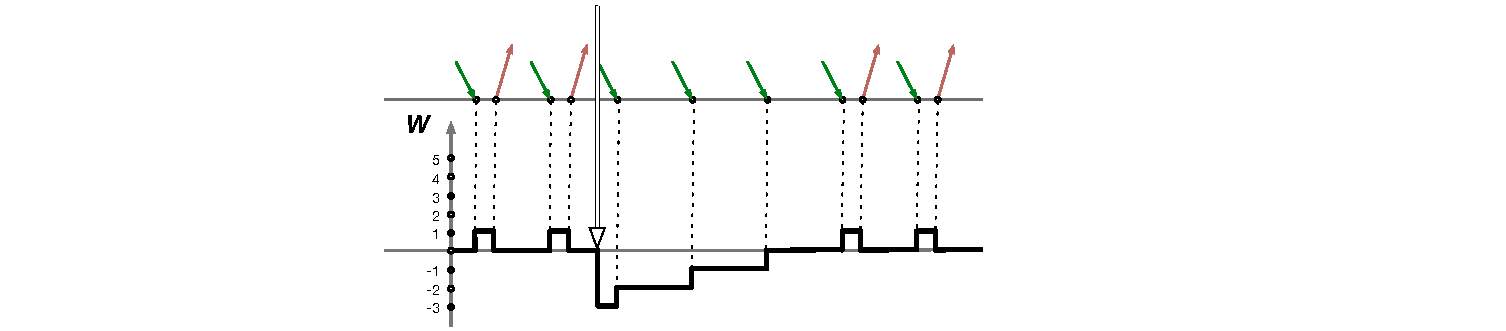
\includegraphics[width=0.35\textwidth]{int-hold}}

\caption{Managing interest expression}
\label{fig:w-concept}
\end{figure}


%%%%%%%


